\documentclass[10pt,a4paper]{article}
\usepackage[utf8]{inputenc}
\usepackage{amsmath}
\usepackage{amsfonts}
\usepackage{amssymb}
\usepackage{graphicx}
\usepackage{cite}
\usepackage{ucs}
\usepackage{listings} %for code
\usepackage{color} %for code
\usepackage{ulem} %dobule underline
\usepackage[english]{babel}
\usepackage[margin=2.5cm]{geometry}
\usepackage[hidelinks]{hyperref}

\author{Stefan Klaus\\stk4@aber.ac.uk\\Aberystwyth, Wales}
\title{Major Project Documentation}

% defines how code will be shown
\definecolor{dkgreen}{rgb}{0,0.6,0}
\definecolor{gray}{rgb}{0.5,0.5,0.5}
\definecolor{mauve}{rgb}{0.58,0,0.82}
% still code
\lstset{frame=tb,
  language=C, %Java
  aboveskip=3mm,
  belowskip=3mm,
  showstringspaces=false,
  columns=flexible,
  basicstyle={\small\ttfamily},
  numbers=none,
  numberstyle=\tiny\color{gray},
  keywordstyle=\color{blue},
  commentstyle=\color{dkgreen},
  stringstyle=\color{mauve},
  breaklines=true,
  breakatwhitespace=true
  tabsize=3
}
\graphicspath{{./figures/}}
%%%%%%%%%%%%%%%%%%%%%%%%%%%%%%%%%%%%%
%	usefull stuff:
%	[3ex] is better than vspace{11pt}
%	\uuline{} gives a double underline
%	
%	\begin{figure}[h]
%	\includegraphics[width = 1\textwidth]{path_to_file}
%	\caption{caption_for_the_picture}
%	\label{Figure 1}
%	\end{figure}
%	
%	centering a small picture
%	\centerline{\includegraphics[width=0.9\textwidth]{file}}
%	
%	start code listing:
%	\begin{lstlisting}
%	\end{lstlisting}
% \textsuperscript{\texttrademark} 
%%%%%%%%%%%%%%%%%%%%%%%%%%%%%%%%%%%%
\begin{document}
\bibliographystyle{IEEEannot}
\maketitle
\newpage
\tableofcontents
\listoffigures
\newpage
\begin{flushleft}
\section{Background and Design}
\subsection{What the Project is about}
This project is about the map building using swarm intelligence.\\
The aspects of the project include SLAM(Simultaneous Localization And Mapping) as well as communication between a swarm of robots.\\
This document will disuse aspects such as robot localisation, deployment of the swarm, communication between robots and environment mapping.\\
My work is based on the research themes in these areas and I am using the robot simulator software Webots\textsuperscript{\texttrademark}. The mobile robot platform I am using is a virtual representation of the E-Puck robot. \\
The Programming will be done in C, using the Webots\textsuperscript{\texttrademark} API.\\[3ex]

One possible scenario for the program I am developing would be the mapping of an environment that would have become partially unknown after e.g. an nature catastrophe. I specify it this way since the team which would deploy this program on their robot swarm would most likely know the estimated size of the target environment, this is important in order to find an appropriate size for the robot swarm.\\
In such an scenario it is not always possible to achieve GPS coverage so the program should at its best function without the need for GPS localisation, so too find a localisation method which does not requires it is key. Another important features of the robot are obviously distance sensors, the E-Puck robot comes equipped with laser distance sensors, which I will use. Other features cover communication possibilities between robots, motor encoders which are needed for moving the robots in a controlled pattern and odometry calculations which will improve the movement and mapping significantly. \\[3ex]
While it is true that the E-puck robot platform is most likely not suitable for such a scenario I use it because of the time limitation for this project and its good integration inside the Webots\textsuperscript{\texttrademark} simulator. 


\subsection{Background}
\subsubsection{SLAM - Simultaneous Localization And Mapping}
The SLAM problem is a current research topic which is based on different localisation algorithms and using a range of different sensor to effectively map an target area. A lot of different approaches have been done and many research papers have been written, the one I am basing my project on being a paper about a SLAM solution designed for autonomous vehicles\cite{Dissanayake2001Solution}.\\
While the research area of this paper is based on a much larger scale and only using 1 vehicle in comparison to flock, it does still give me an insight upon the SLAM problem.\\
E.g. the problem with localisation in an dynamic environment, the paper tackles this problem by using global reference points and a millimetre wave radar, however for my project I do use an static environment and simple laser range finders. So this paper is only used a reference to the localisation problem, especially the idea of using "global" reference points for the created map.\\
As the test environment and the sensors available for the E-puck sensors are limited I will assume that the starting location of the robots is known.\\[3ex]

Another paper I read about this problem used an approach much more similar to my own project, by using different mobile robots which have no GPS access and simply use 2D laser range finders. However the approach described in this paper was based around the mapping of one "lead" robot and the traversing the same map again with a second robot using the map generated by the first for localisation purposes.\\
The second robot would then scan the target area again and refine the already generated map though using the (now stationary) first robot as an reference point. Since my project is planed about using multiple robot which scan the area at the same time it does still gives some information and idea about map sharing and improving. \\
Since my swarm will traverse the area at the same time it would be needed to share the map in real time and know the robot location in comparison to the first global referring point.  By implementing this I could rescan an area if a robot traverse an area another robot already scanned and refine the the final map by this. I will however look into real time sharing between different robots and can not say at this point if I will implement this in my final solution, it is however a interesting thought.\\[3ex]

\subsubsection{Deployment}
The deployment strategy is an important part of my project as it defines how effective the swarm will cover the target area which will define how long it will take to scan and map the whole area. Another important aspect is how many robots can the swarm hold and effectively deploy using the current deployment strategy. \\ 
One research paper I found proposed an solution of a communication network where the comm nodes keep track of the robots positions and guide them in directions which have not been explored in the last time period\cite{Batalin2003Coverage}. The paper uses a solution which is based on small comm nodes deployed by the robot, to make the solution fitting for my project I would have to define some of my E-pucks as communication nodes which remain on a fast position and guide the "scout" E-pucks based on area which have been least visited by the other robots.\\ 
This is certainly an possible solution however it could be considered a waste of robots in an small environment. Since I am using an simulator there is no communication range problem, but as my indentions are to make it as close to a possible real world application as possible I must still consider this.
That is why I am going to implement an maximum communication range for the robots however more about that can be found inside the "Communication" section. It is however an aspect to which I will come back later in my testing.\\[3ex]

Another paper proposed an solution which is based on an Nearest-Neighbour algorithm, meaning every robot must have always a minimum of "N" other robots inside its communication range\cite{Poduri2004Constrained}. In this solution to robots would emit signals to other robots which would manoeuvre the robots away from each other until only "N" robots remain inside the robots communication range. \\
This solution would cover a large area with the swarm fairly fast and also be adaptable for a swarm of any size, however a solution of moving the whole swarm in on direction would be needed in order to cover the whole target area, assuming the robot swarm is not big enough to cover it once completely deployed.
This would therefore need both a lead robot which decides the movement of the swarm and communication robots which would always have at least 1 link to another comm robot in order to have a communication line back to the lead robot. \\
This is one of two 2 deployment strategies I will try to implement during the testing period and try to find out which one would be more fitting for my project.\\[3ex]

\subsubsection{Communication}
While it is possible for me to transfer information easily between robots since I am using a simulator I am still trying implement it as close to a realistic scenario as possible, meaning that the communication range for the robots is limited. In an realistic scenario every robot would have to send the acquired map back to the static start point/lead robot so that an overall map of the environment can be created. \\
Since the communication range for such small robots is limited and can be even further obstructed through obstacles like walls it is important to designated some robots as communication nodes. Such comm nodes would than remain stationary and link the "scout" robots, which do the exploration, back to do the lead robot. \\
Obviously the most effective way to do this is by implementing different behaviour patterns for scouts or comm robots, and implement a decision model which allows the robot to change between either pattern as the needs of the swarm change. E.g. in the start of the exploration no comm robots will be needed as the robots would most likely be inside the comm range of the lead robot, though this may change if the swarm is big and spread out enough. \\[3ex]

To surpass the problems of obstacles obstructing the communication the comm robots would need to position them self on logical places i.e. in order to scan a room it would be important that a comm robot places it self inside, or close to, the doorway so that others can explore the room and still communicated back to the rest of the swarm. The robot would need to stay inside the doorway as signals can not always travel through walls and the energy reserves of mobile robots are limited so they most likely can not send high power signals. \\
I have yet to decide how I am going to implement the communication part of in the project as I am not sure if the E-puck models implemented inside the simulator are able to send signals to other robots. While I know that it is able to transfer signals through the E-puck's laser sensors I do not know if I will implement it as this is fairly difficult and time consuming. I will come back to this should I have enough time available at the end of the project or if no other alternative can be found.\\[3ex]

The theory of what I am going to implement uses a defined maximum communication range for the robots and a grouping strategy which specifies that each scout robot need to stay in contact which at least 1 comm robot while the comm robots always need at least 1 other comm robot inside their communication range. If implemented correctly the comm robots would on this way create a communication link back to the lead robot/starting location which the scout robots can use to transfer all new information back.\\

\begin{figure}[h]
\centering
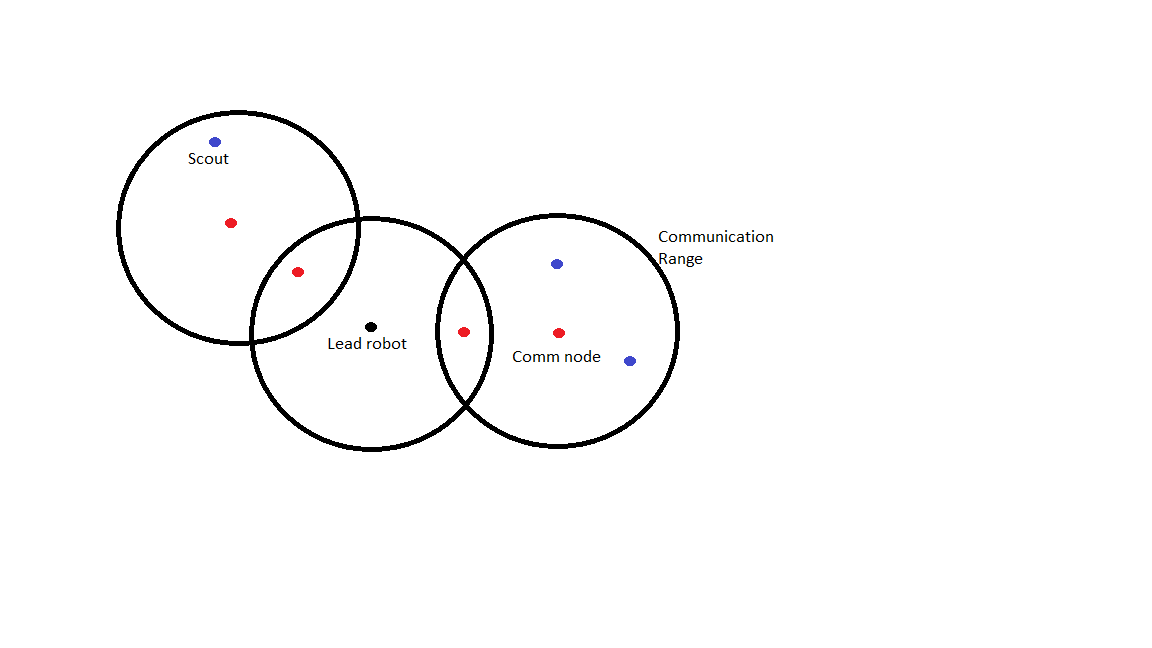
\includegraphics[width = 0.8\textwidth]{figures/comm_example.png} 
\caption{An example of the communication link}
\label{Figure 1}
\end{figure}

Figure 1 shows one possible example of the communication link, where the lead robot/ or in some cases a stationary uplink point is in the center and the communication robots(in red) placed in such positions that their comm range overlaps the comm range of other robots and the lead robot. \\
This configuration allows the scouts(in blue) to move and explore anything inside the communication range of the different comm robots. When the robots at the right side of the figure would now try to move outside the comm range one of them would have to change their behaviour pattern to "communication mode" at the outer range of the other comm nodes range while the last remaining scout continuous exploring in this direction. \\
This example shows that it is important to have a swarm of a suitable size for an environment to be able to cover at much area with the robots at hand and for cases in which this is not possible to be able to move the whole swarm in one unified direction to explore unmapped locations. This is however only doable when there is a lead robot since a stationary comm/uplink point is by definition, stationary.\\

\subsection{Design}
In this section I will describe my design as of the date of the project outline description. \\
This is the design I will follow and try to implement, however this is more of a guideline rather than exact plan since I have to figure out what the API and simulator are able to do and what I am able to implement inside the given time.\\

\subsubsection{Environment Design}
The final environment which I will create for this project will consist of a large starting area, with a corridor adjacent to it. The corridor will hold 1 smaller room to either side, 1 of them with an obstacle inside which will have to be traversed and mapped. The size of the corridor should not be to big so that it is still a challenge to move through it however it should rather not be to small to make movement through it too problematic. \\
A to small size could also make the corridor not distinctive enough from the rest of the wall so the E-Puck could have problem registering and moving into it.\\

\begin{figure}[h]
\centering
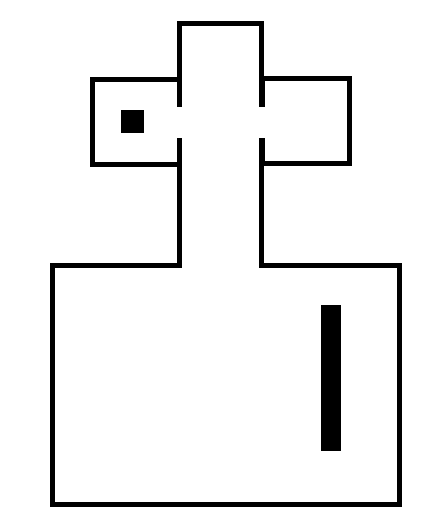
\includegraphics[width=0.5\textwidth]{figures/environment_example.png} 
\caption{Environment Design}
\label{Figure 2}
\end{figure}

\subsubsection{Mapping and Swarm Size}
For mapping I will use a occupancy grid, and the occupancy will be acquired by the E-Puck's laser sensors. 
I will yet have to decide on a resolution, for the grid.\\
I will use a swarm of 5 E-Puck robots, of which 1 will remain stationary and only function as the "Uplink point" to which all robot send the acquired data. 
The stationary robot will also be used as reference point for the localisation method.

\subsubsection{Deployment}
I am of this moment still undecided for which deployment strategy will be implemented. \\
There are 2 deployment strategies which I decided for based on the background research I have done.\\[3ex]

One of them is based on a nearest neighbour approach in which the robots will emit signals to each other which will cause them to drive away from each other until a previous maximum communication distance has been reached. This relationship between robots could be described similar to magnets which can repulse and pull in each other in order to hold a given maximum distance and thereby cover the largest possible area\\
The movement of the robots would be a random walk with included obstacle avoidance. One possibility could be to add a wall following functionality to it as well. However this would require some form of higher functions which to keep the robot from being stuck inside a loop. These higher functions could work by keeping track of the robots position on the map and react once the robot starts traversing the same area again, in this case the algorithm could force to robot back into a random walk.\\[3ex]

The other deployment strategy would implement a more controlled movement pattern. This pattern would move the robots inside a rectangular pattern which would implement a function to move around obstacles on the way before moving back into the original pattern. 
While this reason is more controlled I am not sure which one will turn out to be more effective, that it why I will implement both inside a testing phase and will then decide which of them I will use.

\begin{figure}[h]
\centering
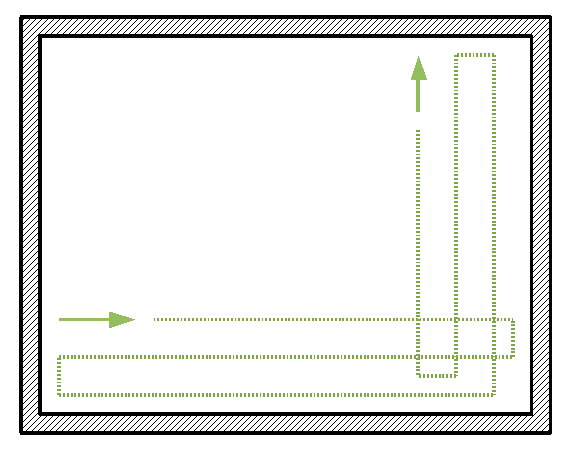
\includegraphics[width=0.5\textwidth]{figures/Trajectory_walk_by_scanning.png}\footnote{url{http://en.wikibooks.org/wiki/File:Trajectory\_walk\_by\_scanning.png}} 
\caption{Movement pattern example}
\label{Figure 3}
\end{figure}

\section{Early Development}
After the first weeks where background reading were done and designing a plan for the final program, I started working with the Webots\textsuperscript{\texttrademark} simulator. \\ More information about the different stages can be found in the following sub-sections. 

\subsection{Webots Tutorials}
In the beginning I was following different tutorials and demo  programs included in the Webots installation. 
This helped me to see how the simulator works, what it can do and what possibilities the Webots API gives me. \\
The tutorials I used were provided by the Webots wikibooks site \footnote{\url{http://en.wikibooks.org/wiki/Cyberbotics\%27_Robot_Curriculum}}.\\
Starting off with simple tutorials and movement and sensor reading I was soon able to implement simple programs which were based on simple forwards movement with obstacle avoidance functions, based on the proximity sensor values. 
After I had done some of the more "advanced"(in comparison to what I had done to this point) tutorials which involved e.g.: reading the robot encoders   I took a look at example programs of more advanced types of movement as well as SLAM examples. \\

\subsection{First Program Iterations}
Taking my experience of the tutorials I moved on to actually implementing the first prototype of my program. \\
The first prototype was still heavily based on a Webots example program called "Intermediate Lawn Mower" which involved a simple movement pattern based on a basic finite state machine(FSM). \\ My first attempt was based recreating the FSM to get the same basic movement capabilities as the the program it was based upon and than changing it to achieve the level of movement control I needed. \\[3ex]

In the following iteration I were trying to implement the functionality of moving a given distance based on resetting the stepper motors encoders and moving the robot until it reaches a given encoder value. I quickly realised that this would not work with the way the FSM was currently implemented so I decided to move the functionality of the FSM, which was currently based on a simple switch statement, to a set of separate functions. The idea was that this would give me the freedom I needed to be able to call a method, i.e. \textit{move\_forward()},  and keep it running until a predefined encoder value has been reached. \\
However this did not work based on the overall way my program was designed at this point. It was designed around an switch statement which based its decisions on the proximity sensors of the E-Puck and then setting the movement speed for the robot motors. As it was based on this calling separate functions to move and turn did not work, which resolved in problems around my current idea of using the stepper motor encoders. \\[3ex] 

As I needed to be able to move a certain distance in order to effectively implement the rectangular movement pattern, I tried various approaches which were all based around the FSM. 
I realised soon that I was not getting anywhere which this way of thinking so I decided to come back to this problem later and went to another problem, turning a given number of degrees. \\
As the simulator simulates friction between the robot wheels and the environment the turning function, as it was in it current state, was far to inaccurate to be usable. \\
It was based on a very basic odometry calculation, taking the encoder values and calculating the turning distance based on the wheel diameter and axle length of the robot. While this is not a bad approach it had no procedures of slowing down the movement as it got closer to the target state so overshooting the wanted position or rotating far to less if the motor speed would have been set to low. \\
I tried countering the problem by alternating the values it used for the odometry calculations, and while I was able to come close a solution it was far from accurate. Another problem with this solution was that it only worked for ~90 degree rotations based on the modified values, meaning all rotations to another point were impossible without modifying the values to fit the target bearing. Which was counter productive as it would be best to have 1 function able to turn the robot to any wanted bearing. \\

\section{Mid stage Development}
After the problems I encountered during my first program iterations, I quickly realised that my way of thinking and understanding of the API was flawed. A lot of the problems I encountered were the result of insufficient programming skills for what I was trying to do combined with bad understanding of how odometry worked, and how I could use it to control the robot.\\
Seeing these kinds of problems I decided to take a step back as I am clearly "moving in circles" and encountering the same kind of problems over and over again with my current approach. \\
I decided to take once more a look at the provided example programs and to study their odometry functions in order to gain some new insight into odometry calculations, and find a new approach based on that.

\subsection{Advanced tutorials}
The example programs provided together with the simulator are categorised after the estimate level of knowledge needed to complete them. Theses categories are: Beginner, Novice, Intermediate and Advanced. I already looked at the advanced programs before as they feature a couple of examples on odometry and slam, however I did not understand it well enough at the time.\\
Looking closer at the odometry functions provided I managed to understand a bit better how the advanced programs worked and how they calculated the movement of the robot. \\[3ex]

I also took a look at the code and notes I took during my Robotics module on the second year, while the API worked different for the Player/Stage environment the idea behind rotation and movement was still the same and had only to be applied using the Webots API.

\subsection{Movement}
After I have studied the odometry functions of the provided programs I decided to start a new approach to fix the movement of the robot.\\
This approach is based on a set of different functions, much smaller and more refined than my previous approach. This approach took a while to implement and test but the results were rather satisfactory. In this section I am going to describe the different aspects of my movement solution and describe how the most important functions work.\\
I will also post the code to each of the major functions as it will help with describing them. 

\subsubsection{Computation of Odometry data} 
The function calculate and return the odometry data works by saving a global buffer of current and previous encoder positions of the stepper motors.
It then calculates how many steps(ticks) the each encoder has done by comparing the previous with the current encoder values. While theses values should remain vaguely the same, since there is friction in the environment small differences will happen, they will be completely different 
when the robot turns. \\
After having calculated the amount of steps taken by each motor it will calculate the distance each wheel has travelled by dividing the number steps by the encoder resolution timed with the wheel radius, where both values have been taken from an example program.
It will then calculate the displacement from the center location by dividing the sum of the distances for the each wheel by 2. And calculate the rotation, theta, by dividing the difference of the distances between the motors with the size of the wheelbase. The wheelbase values has also been taken from another example program.\\
The new X and Y location of the robot can be calculated from the value of the displacement from the center and the current rotation of the robot. 
It will then modify the global buffer for the encoder positions and return an array with the robot's current X and Y location and its rotation.\\
\begin{lstlisting}
/**
Function to compute the robots current odometry data
this includes the x and y placement as well as the rotation theta
*/
double* compute_odometry_data(){
	static double dOdometryData[3];
	double *point_dEncPos;
	
	double dNumTicksLeft = 0.0f;
	double dNumTicksRight = 0.0f;
	double dLeftDist = 0.0f;
	double dRightDist = 0.0f;
	double dDispCenter = 0.0f;
	static double dTheta = 0.0f;
	static double dPosX = 0.0f;
	static double dPosY = 0.0f;
	
	//get encoder position
	point_dEncPos = get_encoder_positions();
	
	/* calculate the distance travled for the wheels
	(number of ticks done since the previous encoder position
	was recoreded)*/
	dNumTicksLeft = point_dEncPos[0] - dPrevEncPos[0];
	dNumTicksRight = point_dEncPos[1] - dPrevEncPos[1];
	
	//convert the number of encoder ticks to a real distance
	dLeftDist = dNumTicksLeft / ENCODER_RESOLUTION * WHEEL_RADIUS;
	dRightDist = dNumTicksRight / ENCODER_RESOLUTION * WHEEL_RADIUS;
	
	//calculate the displacement distance from the center 
	dDispCenter = (dLeftDist + dRightDist)/2.0f;
	
	//calculate the rotation theta of the robot
	dTheta += (dLeftDist - dRightDist)/(WHEELBASE);
	
	//calculate Cartesian coordinates (x, y) of the robot
	dPosX += dDispCenter * sin(dTheta);
	dPosY += dDispCenter * cos(dTheta); 
	
	//update the previous encoder positions
	dPrevEncPos[0] = point_dEncPos[0];
	dPrevEncPos[1] = point_dEncPos[1];
	
	//write the calculate values into the buffer and return
	dOdometryData[0] = dPosX;
	dOdometryData[1] = dPosY;
	dOdometryData[2] = dTheta;
	
	return dOdometryData;
}
\end{lstlisting}

\subsubsection{Moving Forward}
The \textit{move\_forward }function takes 2 doubles as parameters, 1 being the speed with which the robot is ordered to move and the distance it should move.\\
The function first checks that neither of the parameters are 0 and then calculates the number of steps each motor has to drive(1 step being 1 step of the stepper motor) to reach its target position.
This calculation is done by dividing the number of steps needed for a full wheel rotation, 1000 in this case, by the product of $\pi$ times the wheel radius times 2 and multiplication this result with the distance defined in the parameter of the function. The steps needed for a full rotation have been taken from the E-Puck documentation and have been confirmed during on of the odometry tutorials. \\
It will then read the current encoder positions and calculate the stop position for each motor by the sum of the encoder values for each motor and the previously calculated encoder steps needed to reach the target area. 
It will then set the motor speed based on the speed defined in the parameters.\\[3ex]

It then enters the control code which will stop the robot once it reaches it target, position. \\
This is controlled by comparing the current encoder positions with the calculated target encoder positions and updating them all the time. 
Once the robot reached a pre-defined minimum distance of 20 encoder steps it will slow down the movement to a minimum speed of 10 steps per second. This is down to prevent the robot from overshooting the target area should it move with to much speed. The optimal minimum distance and speed has been found experimentally, and both values give good results and also prevent the robot from undershooting.
Once it has reached it target location it will stop the robot, and force the simulator to take a simulation step, effectively moving onward to the next command.\\[3ex]

This function allows me to move forward and stop after the predefined distance within a minimal error space, which will always exist given the friction simulated inside the simulator. This method required a lot of testing in order to get right as first versions did not include the control statement which slowed down the robot after a minimum difference between the encoders and the target encoder value has been reached. So the robot used to overshoot the target. \\
After the control statement was implemented it still required some testing and calibration of the minimum difference and speed values in order to avoid over and undershooting. However the found values work well and the movement error has been reduced to minimum.\\

\begin{lstlisting}
/**
Function to turn the robot a given angle with a given speed
*/
void turn_angle(double dAngle, double dSpeed){
	double dFactor = 0.0f;
	double dStepCount = 0.0f;
	double dStopPosLeft = 0.0f;
	double dStopPosRight = 0.0f;
	double *point_dEncPos;
	
	if((dAngle != 0.0f) && (dSpeed > 0.0f)){
		//calculate turn factor
		dFactor = fabs(360.0f/dAngle);
		
		//calculate the number of step counts for the rotations
		dStepCount = (INCREMENT_STEP * WHEELBASE)/(dFactor * WHEEL_RADIUS * 2.0f);
		
		point_dEncPos = get_encoder_positions();
		
		//turn right
		if(dAngle > 0){
			//calculate the target encoder positions
			dStopPosLeft = point_dEncPos[0] + dStepCount;
			dStopPosRight = point_dEncPos[1] - dStepCount;
			
			point_dOdometryData = compute_odometry_data();
			
			set_motor_speed(dSpeed, -dSpeed);
			
			while((point_dEncPos[0] < dStopPosLeft) && (point_dEncPos[1] > dStopPosRight)){
				//get odometry data
				point_dOdometryData = compute_odometry_data();
				
				//get wheel encoders
				point_dEncPos = get_encoder_positions();
				
				//slow down the closer the robot come to the destination, reduces the error
				if(fabs(dStopPosLeft - point_dEncPos[0]) <= MIN_DIST){
					set_motor_speed(MIN_SPEED, -MIN_SPEED);
				}
			}	
		
	} else { // turn left ...
		dStopPosLeft = point_dEncPos[0] - dStepCount;
		dStopPosRight = point_dEncPos[1] + dStepCount; 

		// turn left the robot ...
		set_motor_speed(-dSpeed, dSpeed);

		while(  (point_dEncPos[0] > dStopPosLeft) &&(point_dEncPos[1] < dStopPosRight)  ) {

			point_dOdometryData = compute_odometry_data();
			point_dEncPos = get_encoder_positions();
			if( fabs(dStopPosLeft - point_dEncPos[0]) <= MIN_DIST ){
				set_motor_speed(-MIN_SPEED, MIN_SPEED); }
			}
		}
	}
	stop_robot();
	
	//update odometry data
	point_dOdometryData = compute_odometry_data();
	wb_robot_step(TIME_STEP);
}
\end{lstlisting}

\subsubsection{Turn a given angle}
The turn\_angle function takes 2 doubles as parameters, one being the angle the robot will turn to the other the speed with which the robot will turn.\\
First the factor by which the robot will turn is calculated by dividing 360, the value of a full rotation, with the defined angle.
Once the factor has been calculated it will then the number of steps the motor have to do until the target position is reached. This is done by dividing the product of the steps needed for a full wheel rotation, 1000, and the size of the wheelbase by the product of the calculated turning factor and 2 times the wheel radius. It will then use a function to return the current motor encoder positions. This function simply uses the Webots\textsuperscript{\texttrademark}  API and returns the values. \\[3ex]

If the rotation angle defined as the function parameter is positive the robot will turn to the right.\\
When the robot is turning to the right it will calculated the stopping positions of the encoders by adding the calculated step count to the left motor encoder and subtracting it from the right encoder. This will lead to the wheels turning against each other and will result in the robot turning on the spot rather than only moving 1 wheel to turn which would result in a displacement of the robot. \\
It will then update the global odometry buffer by calling the \textit{compute\_odometry\_data} function and set the the speed of the motors using the given function parameter value. The right motor will receive a negated value so that it will turn backwards. 
It will then compare the left encoder positions and updated them all the time. Similar to how the forward movement function worked, it will detect when a given minimum difference between the current and target encoder values is reached and slow the robot down to a minimum speed. \\[3ex]

If the rotation angle defined as the function parameter is negative the robot will turn to the left.\\
The only difference between turning left rather than to the right is that the calculations, obviously, are reversed. Meaning to calculated the stop positions of the motor encoders it will subtract the calculated step count from the current left encoder value and add the step count the the right
encoder value, same switch of negation has been done where the motor speeds are set.
The calculations of how long to turn and when to slow down are identical to how they work when turning right, only difference being that the the operators to which check how long to turn are different.\\
Once the target position has been reached, by either turning left or right, the robot stops and the global odometry buffer is updated. 
It will then force to the simulator to take a simulator step, effectively moving on to the next command.\\[3ex]

This functions allows me to define the turn the robot by so many degrees as I need and it will turn there within an minimal error space. This error space exist because the simulator simulates friction between the robot wheels and the environment so 100\% accurate movement will never happen.\\
There also existed the problem of over/undershooting with the turning however the values found during tests of the \textit{move\_forward} function turned out to also work well for the turning function. However one problem remains, since there never is going to be a perfect rotation the error value will add up over time, resulting in less and less accurate turns, overshooting the target rotation is going to be a real problem. I have at this point not yet a solution for this problem, however the function works well and is a great improvement to how it turning was implemented in previous iterations of the program.

\begin{lstlisting}
/**
Function to turn the robot a given angle with a given speed
*/
void turn_angle(double dAngle, double dSpeed){
	double dFactor = 0.0f;
	double dStepCount = 0.0f;
	double dStopPosLeft = 0.0f;
	double dStopPosRight = 0.0f;
	double *point_dEncPos;
	
	if((dAngle != 0.0f) && (dSpeed > 0.0f)){
		//calculate turn factor
		dFactor = fabs(360.0f/dAngle);
		
		//calculate the number of step counts for the rotations
		dStepCount = (INCREMENT_STEP * WHEELBASE)/(dFactor * WHEEL_RADIUS * 2.0f);
		
		point_dEncPos = get_encoder_positions();
		
		//turn right
		if(dAngle > 0){
			//calculate the target encoder positions
			dStopPosLeft = point_dEncPos[0] + dStepCount;
			dStopPosRight = point_dEncPos[1] - dStepCount;
			
			point_dOdometryData = compute_odometry_data();
			
			set_motor_speed(dSpeed, -dSpeed);
			
			while((point_dEncPos[0] < dStopPosLeft) && (point_dEncPos[1] > dStopPosRight)){
				//get odometry data
				point_dOdometryData = compute_odometry_data();
				
				//get wheel encoders
				point_dEncPos = get_encoder_positions();
				
				//slow down the closer the robot come to the destination, reduces the error
				if(fabs(dStopPosLeft - point_dEncPos[0]) <= MIN_DIST){
					set_motor_speed(MIN_SPEED, -MIN_SPEED);
				}
			}	
		
	} else { // turn left ...
		dStopPosLeft = point_dEncPos[0] - dStepCount;
		dStopPosRight = point_dEncPos[1] + dStepCount;
		
		point_dOdometryData = compute_odometry_data();

		// turn left the robot ...
		set_motor_speed(-dSpeed, dSpeed);

		while((point_dEncPos[0] > dStopPosLeft) &&(point_dEncPos[1] < dStopPosRight)){

			point_dOdometryData = compute_odometry_data();
			point_dEncPos = get_encoder_positions();
			if( fabs(dStopPosLeft - point_dEncPos[0]) <= MIN_DIST ){
				set_motor_speed(-MIN_SPEED, MIN_SPEED); }
			}
		}
	}
	stop_robot();
	
	//update odometry data
	point_dOdometryData = compute_odometry_data();
	wb_robot_step(TIME_STEP);
}
\end{lstlisting}

\subsection{Localisation using Odometry}
After the studying the optometry functions provided and implementing the movement algorithms, it was time to implement the localisation using odometry calculations.\\
The odometry functions I implemented are used for localisation the robot inside the environment and finding it heading. The functions only require the starting point and localisation of the robot, and are then apple to calculate the movement and rotation of the robot with every movement done, within a certain degree of accuracy. The uncertainty in accuracy is based on the friction which get simulated inside the simulator. \\
These functions are large similar to the ones provided with the Webots\textsuperscript{\texttrademark} interface, however some minor changes has been done. \\
Similar to the way I have described the movement algorithms I am going to describe the major functions as well as post the code for each function.\\

\subsubsection{Initialising the Odometry algorithms}
To initialize the odometry algorithms, 2 functions are used. \\
The first function, \textit{odometry\_track\_start} takes a \textit{odometrtyTrackStruct}, which is defined in the class which calls the function, as parameter. It will then acquire the encoder positions of the robot and call the next function, \textit{odometry\_track\_start\_pos} which set's the starting values, including the encoder positions inside the odometry struct.\\
\begin{lstlisting}
struct odometryTrackStruct {
	struct {
		float wheel_distance;
		float wheel_conversion;
	} configuration;
	struct {
		int pos_left_prev;
		int pos_right_prev;
	} state;
	struct {
		float x;
		float y;
		float theta;
	} result;
};
 
int odometry_track_start(struct odometryTrackStruct * ot);
int odometry_track_start_pos(struct odometryTrackStruct * ot, double* dEncPos);
void odometry_track_step(struct odometryTrackStruct * ot);
void odometry_track_step_pos(struct odometryTrackStruct * ot, double* dEncPos);
\end{lstlisting}

Also the distance travel when a wheel turns and the wheel conversion are calculated, used for this are parameters acquired during calibrations done in the Webots \textsuperscript{\texttrademark} example programs(the values are the same as it is the same virtual robot model) and the E-Puck documentation. 

\subsubsection{Updating the Odometry values}
To update the odometry values of the struct the function \textit{odometry\_track\_step} is called.
When this function is called inside another function a number of things happen.\\
The current encoder positions for the stepper motors are fetched, 
and used as a parameter inside the \textit{odometry\_track\_step\_pos} function call. \\
Inside this function the new X, Y coordinates and the rotation of the robot are calculated. This is achieved by first calculating the difference between the current encoder positions and the encoder previous encoder positions saved inside the struct. 
This difference is then multiplied by the wheel conversion, which gets calculated inside the initialization step. \\
The result of this is used to calculated the wheel movement of the left and right wheel, results which are used to calculate the rotation of the robot. 
The next step is to calculate the new X and Y coordinates of the robot, based on the sum of done left and right wheel movement  and math calculations using the robots rotation. 
At the end the calculated X and Y coordinates as well as the rotation value are used to update to struct. And the current encoder positions are saved inside the buffer for later calculations. 

\begin{lstlisting}
void odometry_track_step(struct odometryTrackStruct * ot){
	double* point_dEncPos;
	
	point_dEncPos = get_encoder_positions();
	odometry_track_step_pos(ot,	point_dEncPos);
}

void odometry_track_step_pos(struct odometryTrackStruct * ot, double* dEncPos){
	int delta_pos_left, delta_pos_right;
	float delta_left, delta_right, delta_theta, theta2;
	float delta_x, delta_y;
	
	//calculate the difference in position between the previous and current encoder positions. 
	delta_pos_left = dEncPos[0] - ot->state.pos_left_prev;
	delta_pos_right = dEncPos[1] - ot->state.pos_right_prev;
	
	//calculate the rotation based on the displacement of the stepper motors 
	delta_left = delta_pos_left * ot->configuration.wheel_conversion;
	delta_right = delta_pos_right * ot->configuration.wheel_conversion;
	delta_theta = (delta_right - delta_left) / ot->configuration.wheel_distance;
	
	// calculate the x and y displacement 
	theta2 = ot->result.theta + delta_theta * 0.5;
	delta_x = (delta_left + delta_right) * 0.5 *cosf(theta2);
	delta_y = (delta_left + delta_right) * 0.5 * sinf(theta2);
	
	//update the x, y and theta of the struct
	ot->result.x += delta_x;
	ot->result.y += delta_y;
	ot->result.theta += delta_theta;
	
	if(ot->result.theta > M_PI){
		ot->result.theta -= 2*M_PI;
	}
	if(ot->result.theta < -M_PI){
		ot->result.theta += 2*M_PI;
	}
	
	//save current encoder positions to the global buffer 
	ot->state.pos_left_prev = dEncPos[0];
	ot->state.pos_right_prev = dEncPos[1];
}
\end{lstlisting}

\subsection{Implementation}
After these functions were created I tested them using simple test simulations I wrote.\\

\begin{figure}[h]
\centering
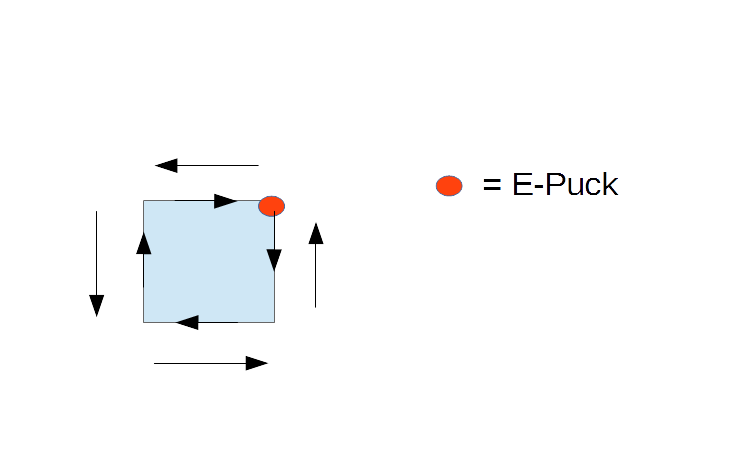
\includegraphics[width = 0.5\textwidth]{figures/movement_test.png} 
\caption{Movement algorithm test pattern}
\label{Figure 4}
\end{figure}

Figure 4 shows a simple movement pattern which I used to calibrate the minimum turn distances and tested that the \textit{move\_forward()} and \textit{turn\_angle()} methods worked as intended. \\
How it works is the E-Puck starts on 1 corner of a square(here I used the floor of the simulator as it has chessboard representation) and move forwards to the other end of the square, turn 90 degrees and so on until it reaches it start point. It then turns around and follows the same pattern back to its original starting position. This tests allows me to notice odometry error in the rotations and forward movement, after a while it would turn/move to far or not far enough and thereby not reach it accurate start point. Noticing these errors allowed me to calibrate my the speed and distance where the algorithms will slow done the movement to minimize this error as much as possible, see section 3.2 for more information on this.\\[3ex]

The accuracy of this test can be increased by using larger movement areas, I used changing 2x2, 4x4 and 3x3 square areas of the chessboard floor to check that my error was at minimal as possible. The test is based on the "University of Michigan Benchmark" or UMBmark\footnote{url{http://www.cs.columbia.edu/~allen/F13/NOTES/borenstein.pdf}}.





\nocite{*}
\newpage
\bibliography{stk4_major_project}
\end{flushleft}
\end{document}

